%!TEX program = xelatex
\documentclass[a4paper,UTF8]{article}
\usepackage{ctex}
\usepackage[margin=1.25in]{geometry}
\usepackage{color}
\usepackage{graphicx}
\usepackage{amssymb}
\usepackage{amsmath}
\usepackage{amsthm}
\usepackage{enumerate}
\usepackage{bm}
\usepackage{hyperref}
\usepackage{epsfig}
\usepackage{color}
\usepackage{mdframed}
\usepackage{lipsum}
\usepackage{graphicx}
\usepackage{float}
\newmdtheoremenv{thm-box}{Theorem}
\newmdtheoremenv{prop-box}{Proposition}
\newmdtheoremenv{def-box}{定义}

\usepackage{listings}
\usepackage{xcolor}
\lstset{
	numbers=left,
	numberstyle= \tiny,
	keywordstyle= \color{ blue!70},
	commentstyle= \color{red!50!green!50!blue!50},
	frame=shadowbox, % 阴影效果
	rulesepcolor= \color{ red!20!green!20!blue!20} ,
	escapeinside=``, % 英文分号中可写入中文
	xleftmargin=2em,xrightmargin=2em, aboveskip=1em,
	framexleftmargin=2em
}

\usepackage{booktabs}

\setlength{\evensidemargin}{.25in}
\setlength{\textwidth}{6in}
\setlength{\topmargin}{-0.5in}
\setlength{\topmargin}{-0.5in}
% \setlength{\textheight}{9.5in}
%%%%%%%%%%%%%%%%%%此处用于设置页眉页脚%%%%%%%%%%%%%%%%%%
\usepackage{fancyhdr}
\usepackage{lastpage}
\usepackage{layout}
\footskip = 12pt
\pagestyle{fancy}                    % 设置页眉
\lhead{2020年秋季}
\chead{神经网络}
% \rhead{第\thepage/\pageref{LastPage}页}
\rhead{作业一}
\cfoot{\thepage}
\renewcommand{\headrulewidth}{1pt}  			%页眉线宽,设为0可以去页眉线
\setlength{\skip\footins}{0.5cm}    			%脚注与正文的距离
\renewcommand{\footrulewidth}{0pt}  			%页脚线宽,设为0可以去页脚线

\makeatletter 									%设置双线页眉
\def\headrule{{\if@fancyplain\let\headrulewidth\plainheadrulewidth\fi%
\hrule\@height 1.0pt \@width\headwidth\vskip1pt	%上面线为1pt粗
\hrule\@height 0.5pt\@width\headwidth  			%下面0.5pt粗
\vskip-2\headrulewidth\vskip-1pt}      			%两条线的距离1pt
 \vspace{6mm}}     								%双线与下面正文之间的垂直间距
\makeatother

%%%%%%%%%%%%%%%%%%%%%%%%%%%%%%%%%%%%%%%%%%%%%%
\numberwithin{equation}{section}
%\usepackage[thmmarks, amsmath, thref]{ntheorem}
\newtheorem{theorem}{Theorem}
\newtheorem*{definition}{Definition}
\newtheorem*{solution}{Solution}
\newtheorem*{prove}{Proof}
\newcommand{\indep}{\rotatebox[origin=c]{90}{$\models$}}

\usepackage{multirow}

%--

%--
\begin{document}
\title{神经网络\\
作业三}
\author{181220076, 周韧哲, zhourz@smail.nju.edu.cn}
\maketitle

\section*{Problem 1}
如下函数适合作为神经网络的激活函数吗?请说明理由。\begin{align*}
	f(x)=\begin{cases}
		0& x<0 \\
		1 & x\geq0
	\end{cases}
\end{align*}
\begin{solution}.\\
	不适合,因为该函数在$x=0$处不可微,在其他定义域的梯度永远为$0$,不适合反向传播来调整误差。
\end{solution}

\begin{figure}
	\centering
	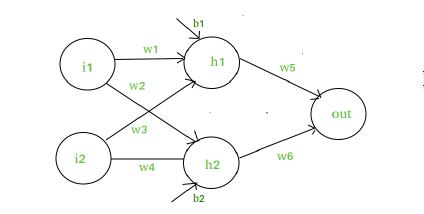
\includegraphics[width=0.7\textwidth]{pics/tmp.png}
	\caption{题2}
	\label{fig:1}
\end{figure}
\section*{Problem 2}
有如下图\ref{fig:1}神经网络,隐藏层使用relu激活函数,输出层使用sigmoid激活函数且没有偏置。对于输入$X_i=\{i_1,i_2\}$,其对应输出记为$Y_i′$,该数据的真实标签记为$Y_i$,这里$i\in\{1,2, ... , n\}$,损失函数定义为
$$E=\sum_{i=1,\cdots,n}(Y_i'-Y_i)^2$$
请推导损失函数对于$w_1,b_2,w_5$的偏导。当$w_1,w_2,w_3,w_4,w_5,w_6$分别取值$0.4,0.5,0.2,0.4,3.5,0.6$且$b1=0.3, b2=0.8$,且只有一条输入数据$X_1=\{ 0.3, 2.8\},Y_1=5.6$的时候,计算该损失函数对于$w_3$的具体值,结果保留两位小数。


\begin{solution}.\\
	令$f_1(x)=Relu(x),f_2(x)=Sigmoid(x)$,且有$f_2'(x)=f_2(x)(1-f_2(x))$,再令
	\begin{align*}
		g(x)=f_1'(x)=\begin{cases}
			0& x\leq0\\
			1& x>0
		\end{cases}
	\end{align*}
	令$E_i=(Y_i'-Y_i)^2$,将网络前向过程写成:
	\begin{align*}
		h_1&=f_1(v_1)=f_1(w_1i_1+w_3i_2+b_1)\\
		h_2&=f_1(v_2)=f_1(w_2i_1+w_4i_2+b_2)\\
		Y_i'&=f_2(v_3)=f_2(w_5h_1+w_6h_2)
	\end{align*}
    则\begin{align*}
    	\frac{\partial E_i}{\partial w_5}&=\frac{\partial E_i}{\partial Y_i'}\frac{\partial Y_i'}{\partial v_3}\frac{\partial v_3}{\partial w_5}=2(Y_i'-Y_i)Y_i'(1-Y_i')h_1\\
    	\frac{\partial E_i}{\partial b_2}&=\frac{\partial E_i}{\partial Y_i'}\frac{\partial Y_i'}{\partial v_3}\frac{\partial v_3}{\partial h_2}\frac{\partial h_2}{\partial v_2}\frac{\partial v_2}{\partial b_2}=2(Y_i'-Y_i)Y_i'(1-Y_i')w_6g(v_2)\\
    	\frac{\partial E_i}{\partial w_1}&=\frac{\partial E_i}{\partial Y_i'}\frac{\partial Y_i'}{\partial v_3}\frac{\partial v_3}{\partial h_1}\frac{\partial h_1}{\partial v_1}\frac{\partial v_1}{\partial w_1}=2(Y_i'-Y_i)Y_i'(1-Y_i')w_5g(v_1)i_1
    \end{align*}
    从而,$$\frac{\partial E}{\partial w_5}=\sum_{i=1}^{n}\frac{\partial E_i}{\partial w_5},\quad\frac{\partial E}{\partial b_2}=\sum_{i=1}^{n}\frac{\partial E_i}{\partial b_2},\quad\frac{\partial E}{\partial w_1}=\sum_{i=1}^{n}\frac{\partial E_i}{\partial w_1}$$
    当只有一条数据时,易知$$\frac{\partial E}{\partial w_3}=\frac{\partial E}{\partial Y_i'}\frac{\partial Y_i'}{\partial v_3}\frac{\partial v_3}{\partial h_1}\frac{\partial h_1}{\partial v_1}\frac{\partial v_1}{\partial w_3}=2(Y_i'-Y_i)Y_i'(1-Y_i')w_5g(v_1)i_2$$
    计算得$v_1=h_1=0.98,v_2=h_2=2.07,v_3=4.672,Y_1'=0.991$,从而得到$$\frac{\partial E}{\partial w_3}=2\times(0.991-5.6)\times0.991\times(1-0.991)\times3.5\times1\times2.8=-0.81$$
\end{solution}
\section*{Problem3}
能否用一个神经元拟合二次曲线?如果能,请给出实例。如果不能,请说明至少需要多少个神经元才能拟合二次曲线。
\begin{solution}.\\
	单个神经元无法拟合二次曲线,至少需要$2$个神经元才能拟合二次曲线,一个隐藏层神经元,一个输出层神经元。只要神经元个数足够多,理论上单隐层的神经网络具有拟合任何函数的能力。
\end{solution}
\end{document}